% !Mode:: "TeX:UTF-8"
% 文字编码:UTF-8
\chapter{引言}
\label{chap:intro}
随着带有摄像功能的便携智能设备的发展,以及各种无线网络覆盖率的提升,视频通话越来越多地应用在人们的日常生活中,如可视电话、视频会议、远程医疗、在线直播等。实时视频传输对网络质量要求较高,而目前无线信道存在的带宽波动、延迟、丢包等问题,使其面临很多困难和挑战。如何提供稳定和高质量的视频服务越来越成为工业界和学术界关注的热点。为此,本课题针对在无线网络上保障实时视频传输的质量,以及提供实用的视频通话服务进行研究。

\section{研究背景及意义}
人类通信的发展经历了飞鸽传书,邮寄信件,电报,固定电话,移动电话等阶段。在互联网出现后,又涌现出Email,网络语音,网络视频等更加方便快捷的通信形式,而移动互联网的发展更使人们随时随地都可以实现语音、视频通信。根据Cisco发布的全球移动数据预测报告\cite{index2016global},过去的2015年中全球移动网络数据流量增长了74\%,达到每个月3.7 艾字节,而到2020年这一数字预计将达到每个月30.6艾字节,人们对于移动互联网的依赖可见一斑。另一方面,如图\ref{fig:cisco_mobile}所示,2015年移动网络数据流量中,视频数据占比重为55\%,到2020年预计为75\%,以62\%的年均增长率成为移动网络中的绝对主流。可以想见,视频通话由于其实效性和丰富的信息量,必将成为人们进行各类通信的最主要方式。与此相应的是,与实时视频服务相关的产品和市场也蓬勃发展起来。日常通信方面,FaceTime、Skype、米聊等内置软件提供的视频聊天功能几乎成了智能手机系统的标配,而QQ、微信、环聊等社交软件也纷纷加入视频聊天功能,以此为基础的小游戏、互动软件也不断被开发出来。在企业全球化的今天,视频电话会议、远程医疗等也成为各大公司必备的生产力工具,具有极大的市场潜力。越来越高清的视频质量和多样化的服务需求,也给实时视频数据的高效传输提出了巨大挑战。

\begin{figure}[htbp]
  \centering
  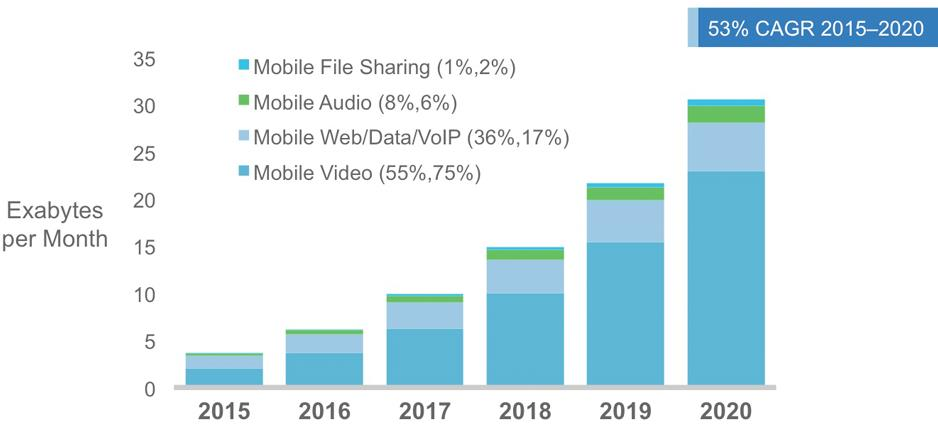
\includegraphics[scale=0.35]{cisco_mobile_traffic.jpg}
  \caption{2020年移动视频流量将占移动总流量的四分之三}
  \label{fig:cisco_mobile}
\end{figure}

高质量的视频体验依赖于较高的视频编解码质量,较低的传输延迟,以及稳定可靠的传输信道。其中任何一项不满足,都会对用户体验造成很大的影响。而在网络传输方面,由于实时性的限制,基于重传的传统TCP协议并不适用于实时视频的传输,大部分实时视频传输都使用了UDP传输协议。而UDP协议并没有对数据传输进行任何保障。无线网络信道的不稳定性,以及终端设备的多样化,也对实时视频的传输优化和质量保证带来了极大挑战。具体来说,在实时视频传输过程中面临的主要问题包括:

\begin{description}
    \item[网络带宽] 视频数据信息量丰富,对网络带宽的需求也很大,如果带宽低于视频最低压缩码率,视频通话将无法进行。同时实时视频传输一般采用的UDP协议本身没有拥塞控制机制,如果应用层没有进行合理限制的话,过高的视频码率将造成网络拥塞,使服务质量急剧下降。而无线网络由于终端位置移动、信号衰减等因素,带宽波动很大。
    \item[延迟] 由于视频通话涉及双方交互,轻微的延迟就会造成明显的通话不连贯。另一方面,为了保证视频播放连续性,每个视频包都需要在相应视频帧播放之前到达,否则就与丢包无异。而无线网络由于信道不稳定,本身存在一定的延迟。并且如果由于带宽波动引发网络拥塞,将产生更大的延迟。
    \item[丢包率] 由于视频文件编码特性,轻微的数据错误都可能造成连续画面的明显失真甚至无法解码。而无线网络下由于信号强度变化、终端移动等,发生数据错误和丢包概率大大增加。
\end{description}

针对以上实时视频传输和无线网络质量之间的一系列矛盾,视频码率自适应和非对称差错保护可以在很大程度上进行改善,具体体现在:

\begin{itemize}
    \item 通过码率自适应算法及时合理地调整视频码率,可以保证网络负载始终稳定在网络承载能力以下,在实现较高带宽利用率的同时避免网络拥塞。既避免了网络拥塞引起延迟增大、丢包等影响视频传输质量的问题,又提高了视频平均码率。
    \item 对于信道不稳定造成的丢包,通过非对称差错保护添加冗余信息,可以为数据传输提供一定容错能力。使视频传输在高丢包环境下也能获得稳定的观看效果。
\end{itemize}

下面我们将介绍我们的算法和系统中涉及到的一些基本概念。

%\subsection{实时视频传输面临的主要挑战和解决方案}
\subsection{实时视频传输基本框架}

\begin{figure}[htbp]
  \centering
  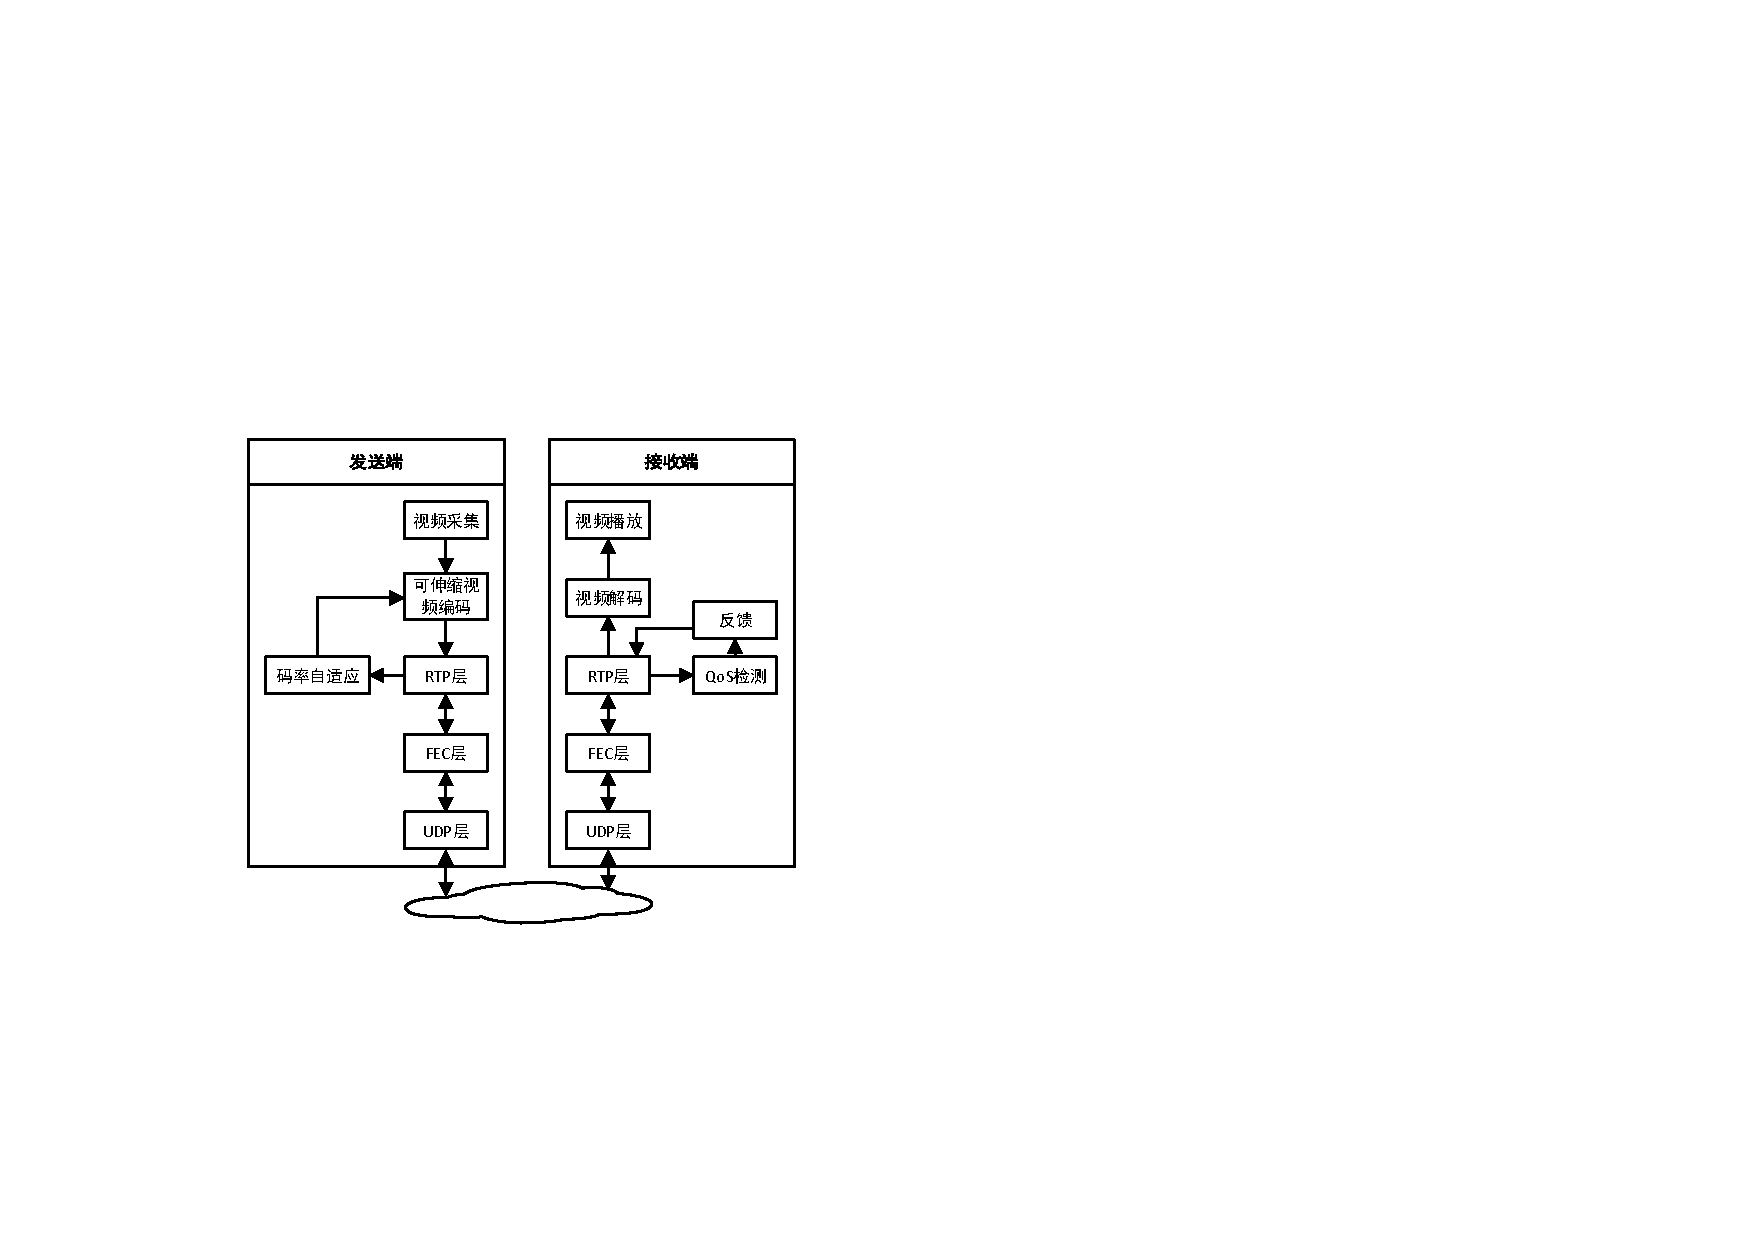
\includegraphics[width=0.7\textwidth]{steaming_architecture.pdf}
  \caption{实时视频传输基本框架图}
  \label{fig:steaming_architecture}
\end{figure}

通常的实时视频传输系统框架如图\ref{fig:steaming_architecture}\cite{wu2000transporting}所示。在发送端,摄像头等视频采集设备将自然场景转换为数字信号;可伸缩视频编码模块对原始视频信号进行编码、压缩等处理,生成码率可变的视频数据流;视频数据需要经过Real-time Transport Protocol(RTP)协议 \cite{jacobson2003rtp} 封装,添加时间戳等信息才能正确地在接收端实时解码;为了应对丢包造成的失真,还可以在发送前对数据包进行FEC编码以添加冗余保护信息(可选);最后,数据由UDP协议封装,通过更底层网络接口发送到接收端。这些数据包可能由于发生拥塞在网络链路上被丢弃,或由于超时而被接收端丢弃。接收端成功接收的数据包,经过一系列拆包、解码,还原为视频图像信息,并按照预定时间戳播放。

注意到视频编码器根据压缩率设置的不同,可以实时生成码率不同的数据流,这也是我们根据网络状况进行视频码率自适应的前提。为了进行码率自适应,在实时视频传输系统框架中一般还加入了位于接收端的Quality of Service(QoS)检测和反馈模块,用于检测当前通信信道的带宽、延迟、丢包率等信息;这些信息通过Real-time Transport Control Protocol(RTCP) 协议 \cite{jacobson2003rtp} 发送给接收端的码率自适应模块,发送端根据不同的码率调整策略改变输出视频的码率。


\subsection{视频码率自适应}
自互联网诞生起,数据传输过程中的速率控制就一直是热门的研究问题。其中TCP协议经过多年改进,现在已经成为网络传输拥塞控制协议的主流。TCP协议通过维护拥塞窗口以及丢包重传机制很好地保障了数据传输的可靠性。然而由于TCP传输过程伴随着较大的延迟,这一协议却并不适用于网络上比重越来越大的实时流媒体传输。实时视频作为一种实时流媒体,与一般网络数据传输最大的不同就是它对数据实时性的要求,一旦数据到达时间超过了有效时间,则与丢包无异。这就要求我们为实时视频传输设计专门的码率自适应算法。

在视频编码过程中,通过设定不同的质量选项,可以动态改变视频数据流的码率。例如在较差的网络条件下使用较低的视频质量,虽然损失了一定的画面清晰度,但是由于数据码率更小,至少能够保证通话过程的平滑流畅。利用这一思路,通过在通话过程中合理地调整视频码率,可以在保证通话顺利进行的前提下,尽可能提高网络带宽利用率,从而获得更好的视频体验。

\subsection{视频传输的非对称差错保护}
实时视频传输和普通文件传输的一个重要区别就是,视频数据即使发生了部分错误,仍然可以继续播放,只是部分画面会出现马赛克或丢帧,降低一定的用户体验。因此在很多视频通话应用中,差错控制模块都属于可选模块。但如果视频传输在高丢包率的网络条件下进行,过多的丢包就会对视频质量造成严重影响,需要通过一定的差错控制措施来减少丢包造成的质量损失。最常用的实时视频传输差错保护方法就是FEC冗余编码。

由于视频编码过程中进行了数据压缩,一个视频流中不同的数据重要性一般是各不相同的。有些数据一旦丢失会造成多个视频帧无法解码,而有些数据只会造成某一帧画面上的少量失真。一种直观的想法是在冗余编码过程中重点保护那些更重要的数据,为它们分配更多的冗余信息。这种根据数据重要程度不同进行不同程度保护的策略成为非对称差错保护。而冗余信息分配是否合理,也在很大程度上影响了冗余保护的效果。


\section{研究内容}
基于上述背景,本次研究的课题选择为面向无线网络的视频通话过程中的拥塞控制、差错保护算法研究,及其在真实软件中的应用。整体研究框架见图\ref{fig:research_architecture},针对无线信道不稳定的特点和实时视频通信对网络的特殊需求,我们的研究主要在以下几个方面展开:首先,为了在保证高效稳定的带宽利用率的前提下尽量避免拥塞和减小通话延迟,我们提出了一种基于延迟优化和控制论模型的视频码率自适应算法;另外,为了减小丢包对视频质量的影响以及传统差错保护算法引入的额外延迟,我们提出了实时视频传输中的非对称差错保护算法优化;最后,基于开源代码实现一个基于上述算法的视频通话应用。本课题希望从这三方面进行研究和系统实现,解决现有实时视频应用系统中存在的问题,提高其服务质量。

\begin{figure}[htbp]
  \centering
  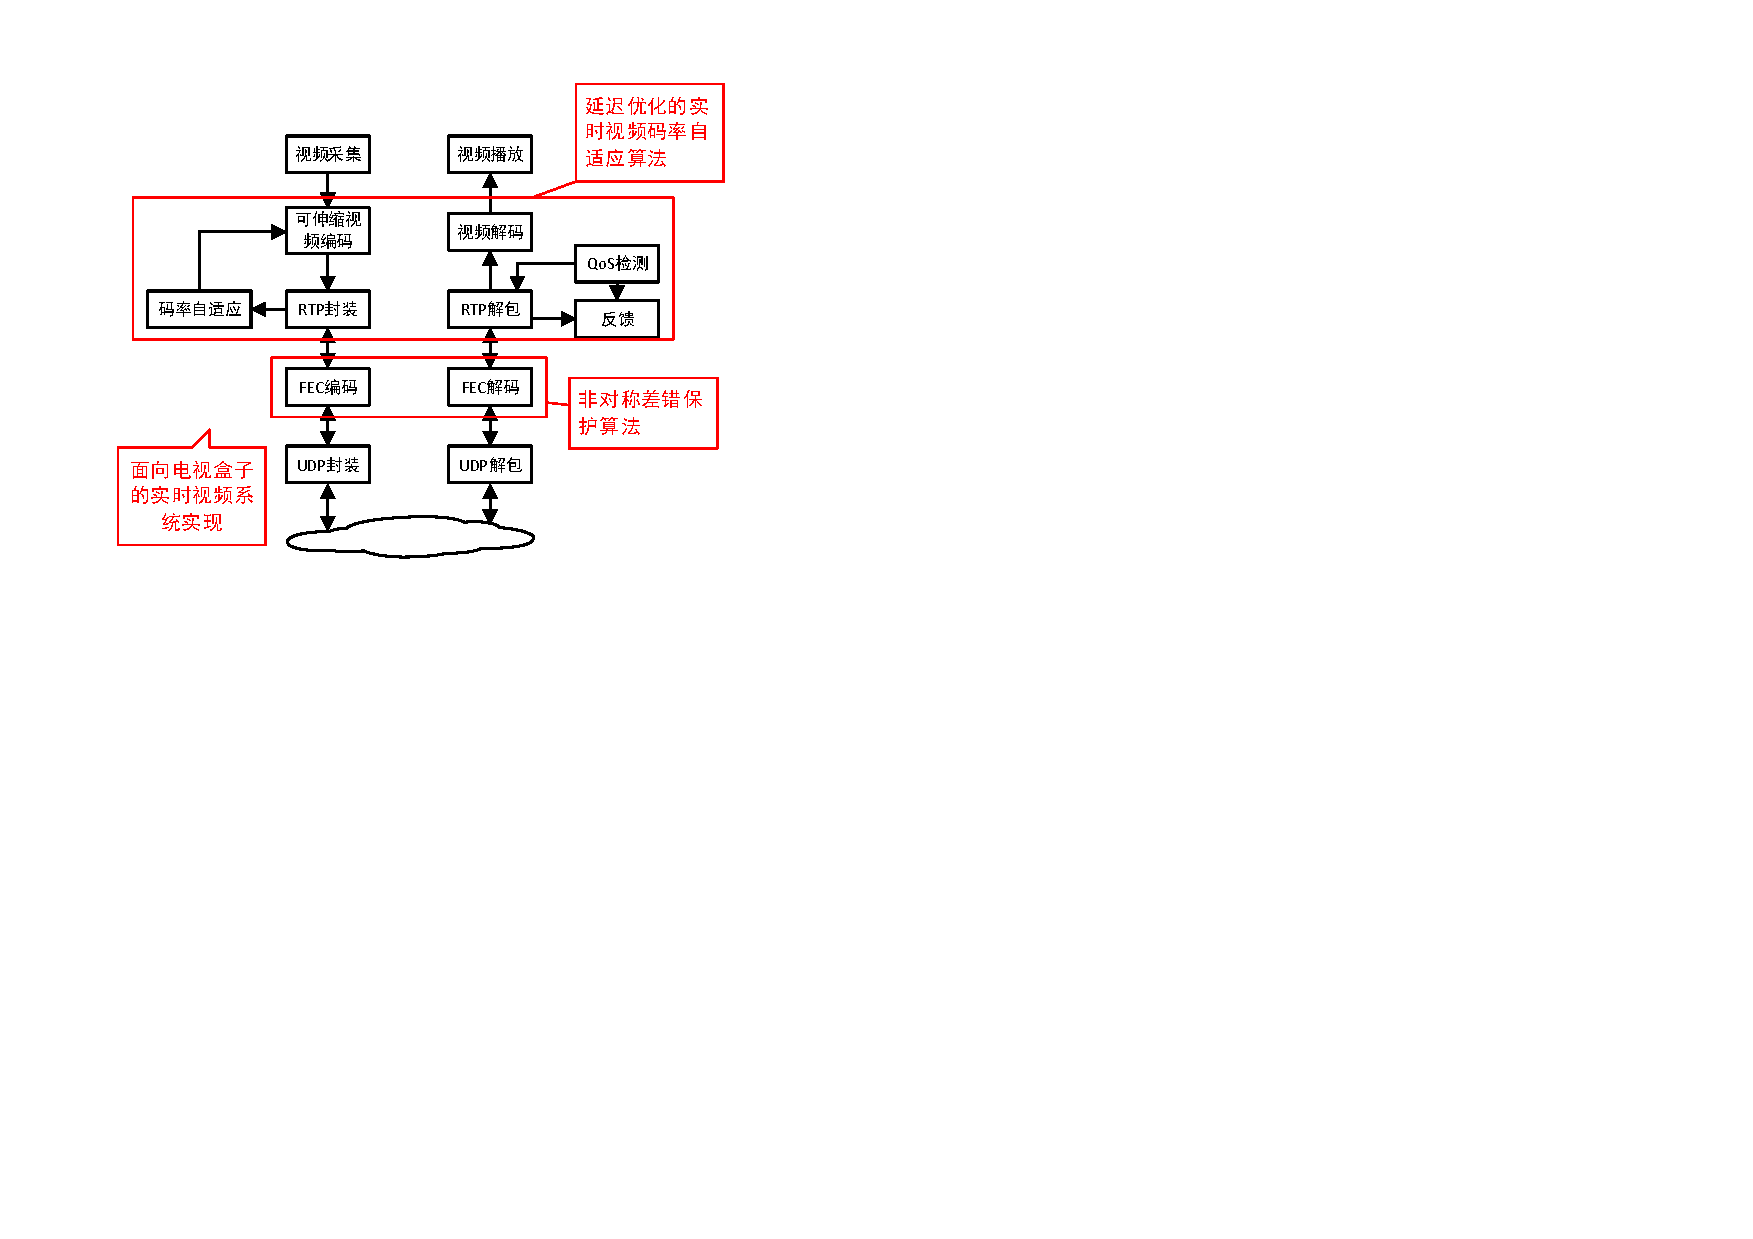
\includegraphics[width=0.8\textwidth]{research_architecture.pdf}
  \caption{研究框架}
  \label{fig:research_architecture}
\end{figure}


\subsection{延迟优化的实时视频码率自适应算法}
高质量的实时视频传输服务要求较大且稳定的带宽、低延迟和低丢包率等,这对于网络拥塞控制也就是视频的码率自适应算法提出了很高的要求。而大部分现有拥塞控制算法主要着眼于避免网络拥塞和整体流量的公平,单个链接获取到的带宽和网络延迟往往都存在很大的波动,这极大降低了实时视频的质量。本研究通过排队延迟模型对网络进行建模,以网络延迟为输入调整视频码率,进而实现稳定高效的带宽利用。另外通过引入控制论模型和PID控制器进行参数优化,进一步提高了视频码率自适应的效果。

\subsection{实时视频传输中的非对称差错保护算法优化}
基于扩展窗口的FEC技术具有不引入额外延迟,控制失真扩散等特点,特别适合无线网络上的实时视频传输。考虑到视频数据的非对称特性,我们可以对差错保护过程进行数学建模,求解最优的冗余信息分配策略,来优化差错保护的效果。而由于扩展窗口的引入,这一优化问题变得层层嵌套,十分复杂,直接求解的难度很大。本研究中,我们针对扩展窗口FEC框架中冗余数据的分配问题进行研究。首先对这一方法进行数学建模,得到一个最优化问题。通过对模型的分析和简化,我们提出了一个简化模型和近似求解方案,成功求解了这一最优分配问题,从而显著提高了视频数据差错保护的效果。

\subsection{面向电视盒子的实时视频通话系统}
在上述算法研究的基础上,本研究在一个开源VOIP软件的基础上进行了底层算法改进和替换,实现了一个视频通话软件。首先在底层RTP和RTCP协议的基础上实现了一个码率自适应模块,根据当前丢包和延迟信息实时调整视频码率。另外,我们还实现了一个独立的差错保护模块,对底层RTP包进行冗余编码和解码,在网络丢包时对视频数据进行恢复,从而更好地适应高丢包率的无线网络环境。最后,考虑到未来视频通话的发展趋势,我们还将这一系统移植到电视盒子上,为家庭用户提供更加高质量的大屏视频通话体验。

\section{论文结构}
本论文的结构安排如下。
第 \ref{chap:intro}章首先介绍了论文的研究背景和意义,以及相关领域面对的挑战。
第 \ref{chap:related}章介绍了实时视频码率自适应和视频流差错保护方面的国内外研究现状。
第 \ref{chap:rate}章以现有拥塞控制算法为基础,考虑实时视频服务对延迟的需求,提出了一种延迟优化的码率自适应算法。
第 \ref{chap:fec}章考虑在易丢包的无线网络下进行视频传输的需求,提出一种视频流非对称差错保护中的冗余分配算法。
综合以上两种算法,我们在第 \ref{chap:system}章设计了一个面向手机和电视盒子的高清视频通话系统。
最后在第 \ref{chap:conclusion}章对本文进行总结和未来工作的展望。
